%
%-----------------------------------
\section{Three-dimensional case}
\label{eq:three-dimensional-case}
%-----------------------------------
%
\begin{figure}[!ht]
	\centering
	\caption{Standard 3D-MOT arrangement}
	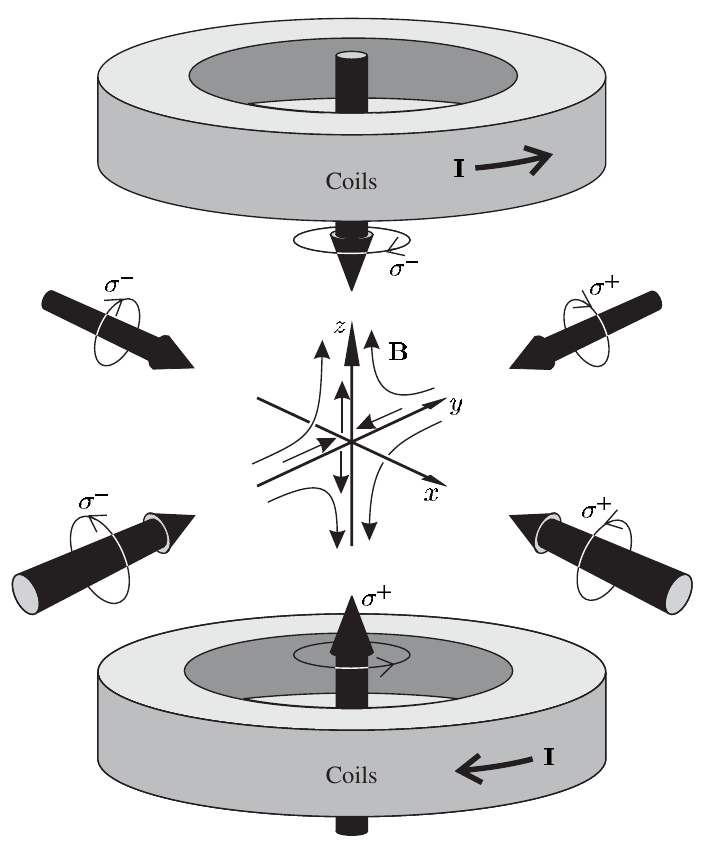
\includegraphics[width=0.5\textwidth]{USPSC-img/standard-3D-MOT-arrangement.png}
	\legend{Standard arrangement of MOT composed of three orthogonal pairs of counter propagating laser beams with opposite circular polarization and coils in anti-Helmholtz configuration, which produces a magnetic quadrupole field. \\ Source: \cite[Figure~9.9]{foot2005atomic}}
	\label{fig:standard-3D-MOT-arrangement}
	\vspace{-20pt}
\end{figure}

Let us assume the standard 3D-MOT arrangement illustrated in figure \ref{fig:standard-3D-MOT-arrangement}. An atom, free to move along all Cartesian axes, interacts with \textit{three pairs} of counter-propagating laser beams with opposite circular polarization and a magnetic quadrupole field $ \mathbf{B} $. In a first attempt, we can naturally extend the 1D-MOT theory into a 3D theory considering that each laser beam yields a radiation pressure force given by equation (\ref{eq:1D-MOT-force-components}). Nevertheless, the quantization axis ($z$-axis) must match the direction of the field $ \mathbf{B} $ to proper evaluate the Zeeman shift, which implies that each laser beam polarization depends on the atomic position. This is not a concern in the 1D-MOT since the magnetic field has a fixed direction. Therefore, a theoretical description of the 3D-MOT \cite{prudnikov2015three} encounters considerable difficult due to the spatial-dependence of the quantization axis. Regardless the theoretical complications, the cooling and trapping effects of MOTs are widely confirmed for many alkali \cite{raab1987trapping, katori1999magneto, zachorowski1998magneto} and lanthanide \cite{maier2014narrow, miyazawa2021narrow, frisch2012narrow}. Also, in this thesis, we could demonstrate both effects for dysprosium and strontium atoms through a Monte Carlo simulation.

%-----------------------------------
\subsection{Limit temperature in Doppler cooling}
\label{sec:Doppler-temperature-limit}
%-----------------------------------

Let us consider a equilibrium atomic position close to the magnetic field centre. In this case, the Zeeman shift becomes negligible compared to the Doppler shift ($ \delta_{Z} \ll \delta_{D} $) such that a defined quantization axis is no longer required. \footnote{Essentially, we are proposing the treatment of a MOT as an \textbf{optical molasses}, which is a similar technique to only cool an atomic dilute gas based upon \textit{Doppler cooling}.} Also, we suppose weak atom-light couplings in which the laser detuning are grater than the power-broadened linewidth. Thus, the interaction between each laser beam and the atom is independent and it is described by two-level dynamics. In this situation, the MOT force is given by
\begin{equation}
	\mathbf{F}_{MOT}(\mathbf{v}) = \frac{\hbar k \Gamma s_0}{2} \sum_{n = 1}^{3} \left( \frac{1}{1 + s_0 + 4[\delta - k (\mathbf{v} \cdot \mathbf{e}_n)]^2 / \Gamma^2} - \frac{1}{1 + s_0 + 4[\delta + k (\mathbf{v} \cdot \mathbf{e}_n)]^2 / \Gamma^2} \right)\mathbf{e}_{n},
\end{equation}
where $ \{ \mathbf{e}_1, \mathbf{e}_2, \mathbf{e}_3 \}$ is the Cartesian basis. We are assuming all laser beams with the same saturation parameter $ s_0 $, wavevector magnitude $ k $, and detuning $ \delta $. For low velocities $ v $ such that $ kv \ll \delta $, we can expand the MOT force around $ \mathbf{v} = 0 $ so that $ \mathbf{F}_{MOT} \simeq - \gamma \mathbf{v} $,
\begin{equation}
	\gamma = - \frac{8 \hbar k^2 s_0 (\delta / \Gamma)}{[1 + s_0 + 4(\delta / \Gamma)^2]^2}.
\end{equation}
Assuming red-detuned laser beams ($ \delta < 0 $), we have $ \gamma > 0 $ and then $ \mathbf{F}_{MOT} $ describes a friction force. Hence, the velocity vanishes after a time as long as $ 1 / \gamma $ and then the final temperature should be zero. However, the $ \mathbf{F}_{MOT} $ is an average. We also must to consider the variance effect of $ \mathbf{F}_{MOT} $ which relies on the Brownian atomic motion due to spontaneous emission. This random dynamics yields a \textit{heating process}. Therefore, the balance between cooling and heating mechanisms set finite temperature.

From the \textit{equipartition theorem}, the average total energy of the atom is given by
\begin{equation}
	\frac{\Delta \mathbf{p}^2}{2m} = \frac{3}{2} k_B T,
\end{equation}
where $ T $ is the temperature of the atomic cloud, $m$ is the the atomic mass, and $ \mathbf{p} $ is the linear momentum of the atom. There is an association between the \textbf{diffusion coefficient}\footnote{Correlation between the $\mathbf{F}_{MOT}(t) $ and $ \mathbf{F}_{MOT}(t + \delta t) $, where $ t $ is a specific instant and $ \delta t $ is a time interval.} $ D $ and the quantity $ \Delta \mathbf{p}^2 $ given by $ \Delta \mathbf{p}^2 \approx D / \gamma $ \cite[Section~2]{perrin2014doppler}. To obtain an expression for $ D $, we need to calculate quantum fluctuations, which is out of the scope of this work. However, skipping this step \cite[Section~2.3]{perrin2014doppler}, there are two possible regimes in which we can define a temperature \cite[Section~V]{loftus2004narrow}:
\begin{itemize}
	\item \textbf{High saturation} ($ s_0 \gg 1 $):
	\begin{equation}
		T(s_0) = \sqrt{s_0} T_0
		\label{eq:Doppler-temperature-high-saturation}
	\end{equation}
	\item \textbf{Low saturation} ($ s_0 \ll 1 $):
	\begin{equation}
		T(s_0, \delta) = \frac{1 + 4(\delta / \Gamma_E)^2}{4|\delta|/\Gamma_E} \sqrt{s_0 + 1} T_0
		\label{eq:Doppler-temperature-low-saturation}
	\end{equation}
\end{itemize}
where $ T_0 \equiv \hbar \Gamma / (2 k_B) $ is known as \textbf{Doppler cooling limit} and $ \Gamma_{E} \equiv \Gamma \sqrt{1 + s_0} $ is the \textbf{power-broadened linewidth}. Considering $ s_0 \gg 1 $ in (\ref{eq:Doppler-temperature-low-saturation}), we obtain (\ref{eq:Doppler-temperature-high-saturation}). The temperature is dependent of the lasers intensity in both regimes and is dependent of the lasers detuning only in the low saturation case. However, making $ \delta \gg 1 $, the temperature of the low saturation case becomes detuning-independent. Indeed, the temperatures in both regimes are equivalent in this limit. Therefore, for high detunings and fixed saturation parameters, we expected a constant temperature.

%-----------------------------------
\subsection{Atomic cloud size}
\label{sec:MOT-cloud-size}
%-----------------------------------

The atomic cloud size is typically characterized by its root-mean-square width along each spatial dimension. There are several factors which influence the cloud size such as the laser arrangement, the magnetic field, the atomic species features, gravity, and interatomic interactions. Overall, the cloud size is defined by the trapping potential. Thus, considering the equipartition theorem, we have
\begin{equation}
	\frac{1}{2} \kappa_{i} \braket{x_i^2} = \frac{1}{2}k_B T
	\Rightarrow \sigma_{i} \equiv \sqrt{\braket{x_i^2}} = \frac{k_B T}{\kappa_{i}} ,
\end{equation}
where $ \sigma_{i} $ is the cloud size on the $ x_i $ direction, $ \kappa_{i} $ is the \textit{spring constant} on the same direction, and $ T $ is the temperature of the cloud. In the unidimensional MOT, from equation (\ref{eq:damped-harmonic-oscillation-1D-MOT}), $ \kappa_{i} = m\omega_{MOT}^2 \propto B_0 / (s_0 \delta)$. Therefore, the more intense the magnetic field gradient, the smaller the cloud size. The saturation parameter and the detuning cause an inverse effect. Assuming a symmetric laser arrangement and the centre of mass at the magnetic field origin, the cloud will have a Gaussian shape with the $ \sigma_z $ smaller by a factor of $ \sqrt{2} $ due to the large magnetic field gradient as shown in figure . In the regime of low density, this is a proper estimation. However, interatomic interactions play a role when the density increases. These interactions expand the cloud by a factor of $ N^{1/3} $ as shown in figure \ref{fig:cloud-size-scaling}, where $ N $ is the number of atoms, due to the reabsorption of scattered photons (light-induced interactions) \cite{PhysRevA.90.063404}. This effect tends to expand the cloud by a factor of $ N^{1/3} $ as shown in figure \ref{fig:cloud-size-scaling}, where $ N $ is the number of atoms.

\begin{figure}[!ht]
    \centering
    \caption{Atomic cloud size scaling in a very large MOT}
    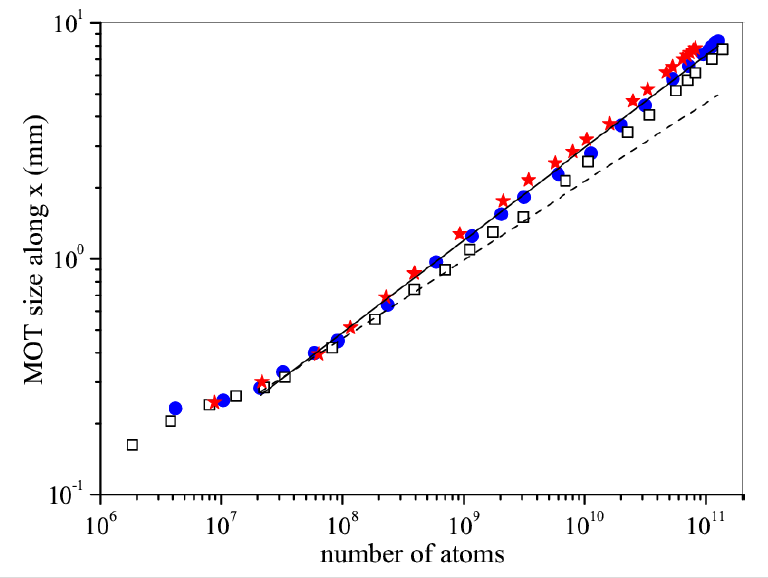
\includegraphics[width=0.6\textwidth]{USPSC-img/atomic-cloud-size-scaling.png}
    \legend{Measure of the full width at half maximum size of a rubidium atomic cloud along the magnetic coils axis. The three sets of data correspond to different MOT detunings. The solid line is a free fit of the data and the dashed line is fit considering the scaling model $ L \propto N^{1/3} $. \\ Source: \cite[Figure~5]{PhysRevA.90.063404}}
    \label{fig:cloud-size-scaling}
    \vspace{-20pt}
\end{figure}

%-----------------------------------
\subsection{Magnetic force}
\label{sec:magnetic-force}
%-----------------------------------

Since the atom experiences a magnetic field gradient, it also feels a position-dependent magnetic force $ \mathbf{F}_B(\mathbf{r}) $ \cite[Section~3.2.1]{courteille2019atom} given by
\begin{equation}
	\mathbf{F}_B(\mathbf{\mathbf{r}}) = - g_J m_J \mu_B \nabla |B(\mathbf{r})|
\end{equation}
where $g_J$ is the \textit{Landé} factor of the ground state and $ m_J $ is the magnetic quantum number of the ground state\footnote{We should consider one force for each excited states. However, the average time $ 1/\Gamma $ that the atom stays in the excited state is much lower than the average time it remains in the ground state.}. The magnetic field $ \mathbf{B}(\mathbf{r}) $ does not have a trivial dependence with the position since it is generated by anti-Helmholtz coils as illustrated in figure \ref{fig:standard-3D-MOT-arrangement}. However, the atom is restricted to move close to the magnetic field centre, otherwise the MOT force will throw it away from the trap. Hence, $ \mathbf{B} $ can be approximated by the following linear expression
\begin{equation}
	\mathbf{B} = B_0 \left(\frac{x}{2} \mathbf{\hat{x}} + \frac{y}{2} \mathbf{\hat{y}} - z \mathbf{\hat{z}} \right),
	\label{eq:magnetic-field-profile}
\end{equation}
where $ B_0 $ depends only on the coils features. Thus, the magnetic force $ \mathbf{F}_B $ will be
\begin{equation}
	\mathbf{F}_B(x, y, z) = - \frac{g_J m_J \mu_B B_0 / 2}{\sqrt{x^2 + y^2 + 4z^2}} \left( x \mathbf{\hat{x}} + y \mathbf{\hat{y}} + 4z \mathbf{\hat{z}} \right),
	\label{eq:magnetic-force-close-to-quadrupole-magnetic-fields-centre}
\end{equation}
where $ x $, $ y $, and $ z $ are the Cartesian coordinates whose origin is the magnetic field. This force is comparable to gravity for very large magnetic field gradients, which is not suitable for MOTs because large gradients decrease the trapping region. Therefore, we expect that the magnetic force will be much lower than the radiation pressure forces.
